\subsubsection{最强检验}\label{sec:8.3.2}
前几节描述了各种假设检验类. 其中一些控制第一类错误概率，例如水平为 $\alpha$ 的检验对所有 $\theta\in\Theta_0$ 都使第一类错误概率不超过 $\alpha$. 这类中的好检验还应具有较小的第二类错误概率，即在 $\theta\in\Theta_0^c$ 时功效函数较大. 若一个检验的第二类错误概率比类中所有其他检验都小，它当然有力地竞争着类中最佳检验的地位. 下列定义将这一想法形式化.
\begin{definition}\label{def:8.3.11}\index{SI0515@一致最强}
设 $\mathscr C$ 是检验 $H_0:\theta\in\Theta_0$ 对 $H_1:\theta\in\Theta_0^c$ 的一个检验类. 类 $\mathscr C$ 中功效函数为 $\beta(\theta)$ 的检验，若对每个 $\theta\in\Theta_0^c$，以及类 $\mathscr C$ 中每个检验的功效函数 $\beta'(\theta)$，都有 $\beta(\theta)\ge\beta'(\theta)$，就称为类 $\mathscr C$ 中的一致最强检验（uniformly most powerful，UMP\mbox{）.}
\end{definition}
本节中，$\mathscr C$ 取全部水平 $\alpha$ 检验构成的类，\autoref{def:8.3.11}中的检验于是称为水平 $\alpha$ 的一致最强检验. 要使这种检验有意义，对 $\mathscr C$ 的限制必须包含对第一类错误概率的某种限制. 完全不控制第一类错误概率而使第二类错误概率最小，并没有多大意义. （例如，以概率 $1$ 拒绝 $H_0$ 的检验永远不会犯第二类错误，见\autoref{exercise:8.16}.）

\autoref{def:8.3.11}要求很强，许多实际问题中不存在一致最强检验. 但在存在时，它完全可以被视为类中最佳检验. 因此，我们希望能识别出存在的一致最强检验. 下面著名的定理明确指出：当原假设和备择假设各自只包含样本的一种概率分布，即二者均为简单假设时\index{SI0480@简单}\semanticindexanchor{480:345}，哪些检验是水平 $\alpha$ 的一致最强检验.
\sourcepageanchor{346}
\begin{theorem}[Neyman–Pearson 引理]\label{thm:8.3.12}\index{SI0722@Neyman–Pearson引理}
考虑检验 $H_0:\theta=\theta_0$ 对 $H_1:\theta=\theta_1$，$\theta_i$ 对应的密度或质量函数为 $f(\boldsymbol x\mid\theta_i)$，$i=0,1$. 使用拒绝域为 $R$ 的检验，满足对某个 $k\ge0$，
\begin{equation}\label{eq:8.3.1}
\begin{aligned}
\boldsymbol x\in R&\quad\text{若 }f(\boldsymbol x\mid\theta_1)>kf(\boldsymbol x\mid\theta_0),\\
\text{且}\qquad\boldsymbol x\in R^c&\quad\text{若 }f(\boldsymbol x\mid\theta_1)<kf(\boldsymbol x\mid\theta_0),
\end{aligned}
\end{equation}
以及
\begin{equation}\label{eq:8.3.2}\alpha=P_{\theta_0}(\boldsymbol X\in R).\end{equation}
则
\begin{enumerate}
\item\phantomsection\label{itm:thm:8.3.12:a}（充分性）任何满足\eqref{eq:8.3.1}和\eqref{eq:8.3.2}的检验，都是水平 $\alpha$ 的一致最强检验.
\item\phantomsection\label{itm:thm:8.3.12:b}（必要性）若存在满足\eqref{eq:8.3.1}、\eqref{eq:8.3.2}且 $k>0$ 的检验，则每个水平 $\alpha$ 的一致最强检验大小都为 $\alpha$（满足\eqref{eq:8.3.2}）；并且每个水平 $\alpha$ 的一致最强检验都满足\eqref{eq:8.3.1}，至多在某个满足 $P_{\theta_0}(\boldsymbol X\in A)=P_{\theta_1}(\boldsymbol X\in A)=0$ 的集合 $A$ 上例外.
\end{enumerate}
\end{theorem}
\begin{proof}
我们证明 $f(\boldsymbol x\mid\theta_0)$ 和 $f(\boldsymbol x\mid\theta_1)$ 是连续随机变量密度的情形. 离散情形的证明只需把积分换成求和（见\autoref{exercise:8.21}\mbox{）.}

首先注意，任何满足\eqref{eq:8.3.2}的检验，大小都为 $\alpha$，从而水平也为 $\alpha$，因为 $\Theta_0$ 只有一个点，故 $\sup_{\theta\in\Theta_0}P_\theta(\boldsymbol X\in R)=P_{\theta_0}(\boldsymbol X\in R)=\alpha$.

为简化记号，定义检验函数（test function）\index{SI1032@检验函数}\semanticindexanchor{1032:346}：它是样本空间上的函数，在 $\boldsymbol x\in R$ 时为 $1$，在 $\boldsymbol x\in R^c$ 时为 $0$，即拒绝域的示性函数. 设 $\phi(\boldsymbol x)$ 是满足\eqref{eq:8.3.1}与\eqref{eq:8.3.2}的检验的检验函数，$\phi'(\boldsymbol x)$ 是任一其他水平 $\alpha$ 检验的检验函数，$\beta(\theta)$ 与 $\beta'(\theta)$ 分别为二者的功效函数. 因为 $0\le\phi'(\boldsymbol x)\le1$，\eqref{eq:8.3.1}蕴含对每个 $\boldsymbol x$，
$$[\phi(\boldsymbol x)-\phi'(\boldsymbol x)][f(\boldsymbol x\mid\theta_1)-kf(\boldsymbol x\mid\theta_0)]\ge0$$
（因为当 $f(\boldsymbol x\mid\theta_1)>kf(\boldsymbol x\mid\theta_0)$ 时 $\phi=1$，当反向严格不等式成立时 $\phi=0$\mbox{）.} 因此，
\begin{equation}\label{eq:8.3.3}
\begin{aligned}
0&\le\int[\phi(\boldsymbol x)-\phi'(\boldsymbol x)][f(\boldsymbol x\mid\theta_1)-kf(\boldsymbol x\mid\theta_0)]\,d\boldsymbol x\\
&=\beta(\theta_1)-\beta'(\theta_1)-k[\beta(\theta_0)-\beta'(\theta_0)].
\end{aligned}
\end{equation}
为证明\hyperref[itm:thm:8.3.12:a]{(a)}，注意 $\phi'$ 的水平为 $\alpha$ 而 $\phi$ 的大小为 $\alpha$，故 $\beta(\theta_0)-\beta'(\theta_0)=\alpha-\beta'(\theta_0)\ge0$. 因而\eqref{eq:8.3.3}与 $k\ge0$ 蕴含
$$0\le\beta(\theta_1)-\beta'(\theta_1)-k[\beta(\theta_0)-\beta'(\theta_0)]\le\beta(\theta_1)-\beta'(\theta_1),$$
表明 $\beta(\theta_1)\ge\beta'(\theta_1)$，即 $\phi$ 的功效不低于 $\phi'$. 因 $\phi'$ 是任意水平 $\alpha$ 的检验，$\theta_1$ 又是 $\Theta_0^c$ 中的唯一点，所以 $\phi$ 是水平 $\alpha$ 的一致最强检验.

为证明\hyperref[itm:thm:8.3.12:b]{(b)}，现令 $\phi'$ 为任一水平 $\alpha$ 的一致最强检验的检验函数. 由\hyperref[itm:thm:8.3.12:a]{(a)}，满足\eqref{eq:8.3.1}和\eqref{eq:8.3.2}的 $\phi$ 也是水平 $\alpha$ 的一致最强检验，故 $\beta(\theta_1)=\beta'(\theta_1)$. 这一事实、\eqref{eq:8.3.3}以及 $k>0$ 蕴含
$$\alpha-\beta'(\theta_0)=\beta(\theta_0)-\beta'(\theta_0)\le0.$$
由于 $\phi'$ 的水平为 $\alpha$，又有 $\beta'(\theta_0)\le\alpha$. 所以 $\beta'(\theta_0)=\alpha$，即 $\phi'$ 的大小为 $\alpha$，且\eqref{eq:8.3.3}此时取等号. 然而，非负被积函数 $[\phi(\boldsymbol x)-\phi'(\boldsymbol x)][f(\boldsymbol x\mid\theta_1)-kf(\boldsymbol x\mid\theta_0)]$ 的积分只有在 $\phi'$ 满足\eqref{eq:8.3.1}时才为零，至多在某个满足 $\int_Af(\boldsymbol x\mid\theta_i)\,d\boldsymbol x=0$ 的集合 $A$ 上例外. 这就证明了\hyperref[itm:thm:8.3.12:b]{(b)}的最后一个断言.
\end{proof}
\sourcepageanchor{347}
下面的推论把 Neyman–Pearson 引理与充分性联系起来.
\begin{corollary}\label{cor:8.3.13}\index{SI0512@充分性}
考虑\autoref{thm:8.3.12}中的假设检验问题. 设 $T(\boldsymbol X)$ 是 $\theta$ 的充分统计量，$g(t\mid\theta_i)$ 是 $T$ 在 $\theta_i$ 下的密度或质量函数，$i=0,1$. 则基于 $T$、拒绝域为 $S$（$T$ 的样本空间的一个子集）的任一检验，只要对某个 $k\ge0$ 满足
\begin{equation}\label{eq:8.3.4}
\begin{aligned}t\in S&\quad\text{若 }g(t\mid\theta_1)>kg(t\mid\theta_0),\\
\text{且}\qquad t\in S^c&\quad\text{若 }g(t\mid\theta_1)<kg(t\mid\theta_0),\end{aligned}
\end{equation}
就是水平 $\alpha$ 的一致最强检验，其中
\begin{equation}\label{eq:8.3.5}\alpha=P_{\theta_0}(T\in S).\end{equation}
\end{corollary}
\begin{proof}
用原样本 $\boldsymbol X$ 表示，基于 $T$ 的检验的拒绝域为 $R=\{\boldsymbol x:T(\boldsymbol x)\in S\}$. 由因子分解定理，可将 $\boldsymbol X$ 的密度或质量函数写为 $f(\boldsymbol x\mid\theta_i)=g(T(\boldsymbol x)\mid\theta_i)h(\boldsymbol x)$，$i=0,1$，其中 $h(\boldsymbol x)$ 非负. 将\eqref{eq:8.3.4}的不等式乘以这一非负函数，就看到 $R$ 满足
$$\boldsymbol x\in R\quad\text{若 }f(\boldsymbol x\mid\theta_1)=g(T(\boldsymbol x)\mid\theta_1)h(\boldsymbol x)>kg(T(\boldsymbol x)\mid\theta_0)h(\boldsymbol x)=kf(\boldsymbol x\mid\theta_0),$$
以及
$$\boldsymbol x\in R^c\quad\text{若 }f(\boldsymbol x\mid\theta_1)=g(T(\boldsymbol x)\mid\theta_1)h(\boldsymbol x)<kg(T(\boldsymbol x)\mid\theta_0)h(\boldsymbol x)=kf(\boldsymbol x\mid\theta_0).$$
另外，由\eqref{eq:8.3.5}，
$$P_{\theta_0}(\boldsymbol X\in R)=P_{\theta_0}(T(\boldsymbol X)\in S)=\alpha.$$
所以，由 Neyman–Pearson 引理的充分性部分，基于 $T$ 的检验是水平 $\alpha$ 的一致最强检验.
\end{proof}
推导满足\eqref{eq:8.3.1}或\eqref{eq:8.3.4}、从而为水平 $\alpha$ 的一致最强检验时，通常把不等式改写为 $f(\boldsymbol x\mid\theta_1)/f(\boldsymbol x\mid\theta_0)>k$ 更方便（须留意除数为零的情形\mbox{）.} 以下例子采用这种方法.
\begin{example}[二项总体的一致最强检验]\label{ex:8.3.14}\index{SI0516@二项}
设 $X\sim\operatorname{binomial}(2,\theta)$. 要检验 $H_0:\theta=1/2$ 对 $H_1:\theta=3/4$. 计算概率质量函数之比，得到
$$\frac{f(0\mid\theta=3/4)}{f(0\mid\theta=1/2)}=\frac14,\qquad
\frac{f(1\mid\theta=3/4)}{f(1\mid\theta=1/2)}=\frac34,\qquad
\frac{f(2\mid\theta=3/4)}{f(2\mid\theta=1/2)}=\frac94.$$
选择 $3/4<k<9/4$，Neyman–Pearson 引理说明，在 $X=2$ 时拒绝 $H_0$ 的检验是水平 $\alpha=P(X=2\mid\theta=1/2)=1/4$ 的一致最强检验. 选择 $1/4<k<3/4$，引理说明，在 $X=1$ 或 $2$ 时拒绝 $H_0$ 的检验是水平 $\alpha=P(X=1\text{ 或 }2\mid\theta=1/2)=3/4$ 的一致最强检验. 取 $k<1/4$ 或 $k>9/4$，分别得到水平 $\alpha=1$ 或 $\alpha=0$ 的一致最强检验.

注意，若 $k=3/4$，\eqref{eq:8.3.1}要求在样本点 $x=2$ 时拒绝 $H_0$，在 $x=0$ 时接受 $H_0$，但未决定 $x=1$ 时采取何种行动. 若在 $x=1$ 时接受 $H_0$，就得到上面水平 $\alpha=1/4$ 的一致最强检验；若在 $x=1$ 时拒绝 $H_0$，就得到水平 $\alpha=3/4$ 的一致最强检验.
\end{example}
\autoref{ex:8.3.14}还说明，在离散分布情形，检验所能达到的 $\alpha$ 水平取决于具体的概率质量函数. （连续情形没有这种问题，任意 $\alpha$ 水平都可达到.）
\sourcepageanchor{348}
\begin{example}[正态总体的一致最强检验]\label{ex:8.3.15}\index{SI0517@正态}
设 $X_1,\ldots,X_n$ 是来自 $\mathrm n(\theta,\sigma^2)$ 总体的随机样本，$\sigma^2$ 已知. 样本均值 $\bar X$ 是 $\theta$ 的充分统计量. 考虑检验 $H_0:\theta=\theta_0$ 对 $H_1:\theta=\theta_1$，其中 $\theta_0>\theta_1$. \eqref{eq:8.3.4}中的不等式 $g(\bar x\mid\theta_1)>kg(\bar x\mid\theta_0)$ 等价于
$$\bar x<\frac{(2\sigma^2\log k)/n-\theta_0^2+\theta_1^2}{2(\theta_1-\theta_0)}.$$
这里利用了 $\theta_1-\theta_0<0$. 随着 $k$ 从 $0$ 增至 $\infty$，右端从 $-\infty$ 增至 $\infty$.\footnote{译注：按所写公式，分母 $2(\theta_1-\theta_0)<0$，故右端实际上随 $k$ 增大而从 $+\infty$ 减至 $-\infty$. 原文方向颠倒，但右端能遍历所有实数及后续检验结论不受影响.} 因此，由\autoref{cor:8.3.13}，拒绝域为 $\bar x<c$ 的检验是水平 $\alpha$ 的一致最强检验，其中 $\alpha=P_{\theta_0}(\bar X<c)$. 若指定某个 $\alpha$，则一致最强检验在 $\bar X<c=-\sigma z_\alpha/\sqrt n+\theta_0$ 时拒绝 $H_0$. 如此选择 $c$ 保证\eqref{eq:8.3.5}成立.
\end{example}
像 Neyman–Pearson 引理中的 $H_0,H_1$ 那样，仅为样本 $\boldsymbol X$ 指定一种可能分布的假设，称为简单假设（simple hypotheses\mbox{）.}\index{SI0480@简单}\semanticindexanchor{480:348} 多数实际问题中，所关心的假设为样本指定不止一种可能分布，这种假设称为复合假设（composite hypotheses\mbox{）.}\index{SI0476@复合}\semanticindexanchor{476:348} 由于\autoref{def:8.3.11}要求一致最强检验对每个单独的 $\theta\in\Theta_0^c$ 都最强，因此可以用 Neyman–Pearson 引理寻找复合假设问题中的一致最强检验.

特别地，断言一元参数较大（如 $H:\theta\ge\theta_0$）或较小（如 $H:\theta<\theta_0$）的假设，称为单侧假设（one-sided hypotheses\mbox{）.}\index{SI0478@单侧}\semanticindexanchor{478:348} 断言参数或者较大或者较小（如 $H:\theta\ne\theta_0$）的假设，称为双侧假设（two-sided hypotheses\mbox{）.}\index{SI0481@双侧}\semanticindexanchor{481:348} 一大类具有水平 $\alpha$ 一致最强检验的问题，涉及单侧假设以及具有单调似然比性质的密度或质量函数.
\begin{definition}\label{def:8.3.16}\index{SI0700@单调似然比}
对一元随机变量 $T$ 及实值参数 $\theta$，若密度或质量函数族 $\{g(t\mid\theta):\theta\in\Theta\}$ 满足：对每个 $\theta_2>\theta_1$，比值 $g(t\mid\theta_2)/g(t\mid\theta_1)$ 在 $\{t:g(t\mid\theta_1)>0\text{ 或 }g(t\mid\theta_2)>0\}$ 上是 $t$ 的单调函数（非增或非减），则称该族具有单调似然比（monotone likelihood ratio，MLR\mbox{）.} 注意，对 $c>0$，规定 $c/0=\infty$.
\end{definition}
许多常见分布族具有单调似然比，例如正态族（方差已知、均值未知）、泊松族和二项族. 事实上，若 $w(\theta)$ 是非减函数，则任意正则指数族 $g(t\mid\theta)=h(t)c(\theta)e^{w(\theta)t}$ 都具有单调似然比（见\autoref{exercise:8.25}\mbox{）.}
\begin{theorem}[Karlin–Rubin]\label{thm:8.3.17}\index{SI0594@Karlin–Rubin定理}
考虑检验 $H_0:\theta\le\theta_0$ 对 $H_1:\theta>\theta_0$. 设 $T$ 是 $\theta$ 的充分统计量，且 $T$ 的密度或质量函数族 $\{g(t\mid\theta):\theta\in\Theta\}$ 具有单调似然比. 则对任意 $t_0$，当且仅当 $T>t_0$ 时拒绝 $H_0$ 的检验，是水平 $\alpha=P_{\theta_0}(T>t_0)$ 的一致最强检验.\footnote{译注：本定理和下述证明实际需要似然比关于 $t$ 非减，而前面的定义同时允许非增. 若似然比非增，拒绝域方向应相应反转；例如 $X\sim\mathrm n(\theta,1)$ 而 $T=-X$ 时，似然比关于 $T$ 非增，$P_\theta(T>t_0)$ 随 $\theta$ 下降，不能直接套用本述. 正文保留原假设.}
\end{theorem}
\begin{proof}
设 $\beta(\theta)=P_\theta(T>t_0)$ 为检验的功效函数. 固定 $\theta'>\theta_0$，考虑检验 $H'_0:\theta=\theta_0$ 对 $H'_1:\theta=\theta'$. 由于 $T$ 的密度或质量函数族具有单调似然比，$\beta(\theta)$ 非减（\autoref{exercise:8.34}），因此
\begin{enumerate}[label=\roman*.]
\item\phantomsection\label{itm:proof:8.3.17:i} $\sup_{\theta\le\theta_0}\beta(\theta)=\beta(\theta_0)=\alpha$，故这是一个水平 $\alpha$ 的检验.
\item\phantomsection\label{itm:proof:8.3.17:ii} 定义
$$k'=\inf_{t\in\mathscr T}\frac{g(t\mid\theta')}{g(t\mid\theta_0)},$$
其中 $\mathscr T=\{t:t>t_0\text{ 且 }g(t\mid\theta')>0\text{ 或 }g(t\mid\theta_0)>0\}$，则\footnote{译注：这里的 $\mathscr T$ 按原文意思应读作 $t>t_0$ 且两个密度至少一个为正. 此外，“$\Longleftrightarrow$”及右端严格“$>$”一般不成立：离散分布可能在最小拒绝点达到该下确界，非严格单调的比值也可能有平台. 证明只需核验 Neyman–Pearson 的两个严格不等式所规定的方向，并在比值等于临界值处采用所需的拒绝规则；还应在同一自变量 $t=T$ 下读该式.}
$$T>t_0\ \Longleftrightarrow\ \frac{g(t\mid\theta')}{g(t\mid\theta_0)}>k'.$$
\end{enumerate}

结合\autoref{cor:8.3.13}，\hyperref[itm:proof:8.3.17:i]{(i)} 与\hyperref[itm:proof:8.3.17:ii]{(ii)} 蕴含 $\beta(\theta')\ge\beta^*(\theta')$，其中 $\beta^*(\theta)$ 是 $H'_0$ 的任一其他水平 $\alpha$ 检验的功效函数，即满足 $\beta(\theta_0)\le\alpha$ 的任一检验.\footnote{译注：此处原文写 $\beta(\theta_0)\le\alpha$，依上下文正在描述其他检验，宜为 $\beta^*(\theta_0)\le\alpha$；保留原记号.} 然而，$H_0$ 的任一水平 $\alpha$ 检验都满足 $\beta^*(\theta_0)\le\sup_{\theta\in\Theta_0}\beta^*(\theta)\le\alpha$. 因此对 $H_0$ 的任一水平 $\alpha$ 检验都有 $\beta(\theta')\ge\beta^*(\theta')$. 由于 $\theta'$ 任意，原检验是水平 $\alpha$ 的一致最强检验.
\end{proof}
\sourcepageanchor{349}
类似论证表明，在\autoref{thm:8.3.17}的条件下，当且仅当 $T<t_0$ 时拒绝 $H_0:\theta\ge\theta_0$、支持 $H_1:\theta<\theta_0$ 的检验，是水平 $\alpha=P_{\theta_0}(T<t_0)$ 的一致最强检验.
\begin{example}[续\autoref{ex:8.3.15}]\label{ex:8.3.18}\index{SI0517@正态}
考虑检验 $H'_0:\theta\ge\theta_0$ 对 $H'_1:\theta<\theta_0$，采用在
$$\bar X<-\frac{\sigma z_\alpha}{\sqrt n}+\theta_0$$
时拒绝 $H'_0$ 的检验. 因 $\bar X$ 充分，且其分布具有单调似然比（\autoref{exercise:8.25}），由\autoref{thm:8.3.17}可知，这是该问题中水平 $\alpha$ 的一致最强检验.

该检验的功效函数
$$\beta(\theta)=P_\theta\left(\bar X<-\frac{\sigma z_\alpha}{\sqrt n}+\theta_0\right)$$
是 $\theta$ 的减函数（$\theta$ 是 $\bar X$ 分布的位置参数），因此 $\alpha$ 由 $\sup_{\theta\ge\theta_0}\beta(\theta)=\beta(\theta_0)=\alpha$ 给出.
\end{example}
虽然多数实验者若知道一个水平 $\alpha$ 的一致最强检验，就会选择使用它，但遗憾的是许多问题中并不存在这样的检验. 原因是水平 $\alpha$ 的检验类太大，没有一个检验在功效上优于所有其他检验. 此时，继续寻找好检验的常见方法是考虑这一检验类的某个子集，尝试在子集中找到一致最强检验. 这应使人想起\autoref{sec:7}：为研究最优性，我们把范围限制在无偏点估计量中. 下面说明，把范围限制在无偏检验组成的子集，如何帮助找到最佳检验.

首先考虑一个例子，说明水平 $\alpha$ 的一致最强检验不存在的一种典型情况.
\begin{example}[一致最强检验的不存在性]\label{ex:8.3.19}
设 $X_1,\ldots,X_n$ 独立同分布于 $\mathrm n(\theta,\sigma^2)$，$\sigma^2$ 已知. 考虑检验 $H_0:\theta=\theta_0$ 对 $H_1:\theta\ne\theta_0$. 对指定的 $\alpha$，本问题中水平 $\alpha$ 的检验就是满足
\begin{equation}\label{eq:8.3.6}P_{\theta_0}(\text{拒绝 }H_0)\le\alpha\end{equation}
的任一检验.

考虑备择参数点 $\theta_1<\theta_0$. \autoref{ex:8.3.18}的分析表明，在满足\eqref{eq:8.3.6}的全部检验中，若 $\bar X<-\sigma z_\alpha/\sqrt n+\theta_0$ 则拒绝 $H_0$ 的检验，在 $\theta_1$ 处有最高功效. 称其为检验1. 而且，由 Neyman–Pearson 引理的\hyperref[itm:thm:8.3.12:b]{(b)（必要性）}，任何在 $\theta_1$ 处达到同样高功效的其他水平 $\alpha$ 检验，必须具有与检验1相同的拒绝域，至多相差一个满足 $\int_A f(\boldsymbol x\mid\theta_i)\,d\boldsymbol x=0$ 的集合 $A$. 所以，若本问题存在水平 $\alpha$ 的一致最强检验，它必须是检验1，因为没有其他检验在 $\theta_1$ 处具有同样高的功效.

现在考虑检验2：若 $\bar X>\sigma z_\alpha/\sqrt n+\theta_0$ 则拒绝 $H_0$. 检验2的水平也是 $\alpha$. 记 $\beta_i(\theta)$ 为检验 $i$ 的功效函数. 对任意 $\theta_2>\theta_0$，
$$\begin{aligned}
\beta_2(\theta_2)&=P_{\theta_2}\left(\bar X>\frac{\sigma z_\alpha}{\sqrt n}+\theta_0\right)\\
&=P_{\theta_2}\left(\frac{\bar X-\theta_2}{\sigma/\sqrt n}>z_\alpha+\frac{\theta_0-\theta_2}{\sigma/\sqrt n}\right)\\
&>P(Z>z_\alpha)&&\text{（$Z\sim\mathrm n(0,1)$，$\theta_0-\theta_2<0$）}\\
&=P(Z<-z_\alpha)\\
&>P_{\theta_2}\left(\frac{\bar X-\theta_2}{\sigma/\sqrt n}<-z_\alpha+\frac{\theta_0-\theta_2}{\sigma/\sqrt n}\right)&&\text{（仍因 $\theta_0-\theta_2<0$）}.
\end{aligned}$$
\sourcepageanchor{350}

\begin{figure}[htbp]\centering
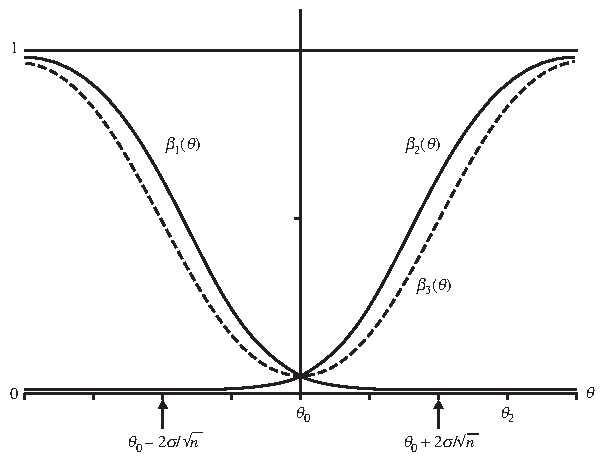
\includegraphics[width=.83\textwidth]{assets/chapter8/fig8-3-3.pdf}
\caption{\autoref{ex:8.3.19}中三个检验的功效函数. $\beta_3(\theta)$ 是一个无偏的水平 $\alpha=.05$ 检验的功效函数.}\label{fig:8.3.3}
\end{figure}

上式最后一项等于
$$P_{\theta_2}\left(\bar X<-\frac{\sigma z_\alpha}{\sqrt n}+\theta_0\right)=\beta_1(\theta_2).$$
所以检验1不是水平 $\alpha$ 的一致最强检验，因为检验2在 $\theta_2$ 处的功效更高. 前面又已证明，如果存在水平 $\alpha$ 的一致最强检验，它必为检验1. 因此本问题不存在水平 $\alpha$ 的一致最强检验.\footnote{译注：这里的不存在性结论针对非平凡水平 $0<\alpha<1$，也是上述有限正态临界点论证的适用范围. 端点 $\alpha=0$ 或 $1$ 有相应的平凡一致最强检验.}
\end{example}
\autoref{ex:8.3.19}再次说明 Neyman–Pearson 引理的用途. 先前用其充分性部分构造水平 $\alpha$ 的一致最强检验；要说明这种检验不存在，则使用其必要性部分.
\begin{example}[无偏检验]\label{ex:8.3.20}
当全部检验类中没有水平 $\alpha$ 的一致最强检验时，可以尝试在无偏检验类中寻找. 检验3当且仅当
$$\bar X>\sigma z_{\alpha/2}/\sqrt n+\theta_0\quad\text{或}\quad\bar X<-\sigma z_{\alpha/2}/\sqrt n+\theta_0$$
时，拒绝 $H_0:\theta=\theta_0$、支持 $H_1:\theta\ne\theta_0$. 其功效函数 $\beta_3(\theta)$ 与\autoref{ex:8.3.19}中的 $\beta_1(\theta),\beta_2(\theta)$ 一起画在\autoref{fig:8.3.3}中. 检验3事实上是水平 $\alpha$ 的一致最强无偏检验，即在无偏检验类中一致最强.

注意，虽然检验1和检验2在某些参数点的功效略高于检验3，但在其他参数点，检验3的功效比检验1和检验2高得多. 例如，$\beta_3(\theta_2)$ 接近一，而 $\beta_1(\theta_2)$ 接近零. 若希望在 $\theta$ 偏大或偏小时都拒绝 $H_0$，\autoref{fig:8.3.3}表明，整体而言检验3优于检验1或检验2.
\end{example}
